\documentclass[12pt,a4paper]{report}

% Packages
\usepackage{geometry}
\usepackage{fancyhdr}   
\usepackage{setspace}
\usepackage{titlesec}
\usepackage{graphicx}
\usepackage{lipsum} 
\usepackage{caption}
\usepackage{xcolor}
\usepackage{listings}
\usepackage{textcomp}
\usepackage{amsmath,amssymb}
\usepackage{tikz}
\usepackage{float}
\usetikzlibrary{shapes.geometric, arrows.meta, positioning}
\usepackage{mdframed}
\usepackage{url}
\usepackage[hidelinks]{hyperref}

\definecolor{mGreen}{rgb}{0,0.6,0}
\definecolor{mGray}{rgb}{0.5,0.5,0.5}
\definecolor{mPurple}{rgb}{0.58,0,0.82}
\definecolor{backgroundColour}{rgb}{0.95,0.95,0.92}
\definecolor{codebg}{RGB}{245, 247, 250}
\definecolor{codeframe}{RGB}{200, 210, 220}

% Set page margins
\geometry{top=1in, bottom=1in, left=1in, right=1in}

% Page numbering format
\pagestyle{fancy}
\fancyhf{}
\rfoot{\thepage}
\renewcommand{\headrulewidth}{0pt}

% Chapter and Section formatting
\titleformat{\chapter}[display]
  {\normalfont\fontsize{14}{16}\selectfont\bfseries\centering}{\MakeUppercase{\chaptertitlename}\ \thechapter}{20pt}{\fontsize{14}{16}\selectfont\bfseries}
\titleformat{\section}
  {\normalfont\fontsize{12}{14}\selectfont\bfseries}{\thesection}{1em}{}
\titleformat{\subsection}
  {\normalfont\fontsize{12}{14}\selectfont\bfseries}{\thesubsection}{1em}{}
\titleformat{\subsubsection}
  {\normalfont\fontsize{12}{14}\selectfont\bfseries}{\thesubsubsection}{1em}{}

% Table of Contents formatting
\makeatletter
\renewcommand*\l@chapter[2]{%
  \ifnum \c@tocdepth >\m@ne
    \addpenalty{-\@highpenalty}%
    \vskip 1.0em \@plus\p@
    \setlength\@tempdima{1.5em}%
    \begingroup
      \parindent \z@ \rightskip \@pnumwidth
      \parfillskip -\@pnumwidth
      \leavevmode \bfseries
      \advance\leftskip\@tempdima
      \hskip -\leftskip
      #1\nobreak\hfil \nobreak\hb@xt@\@pnumwidth{\hss #2}\par
      \penalty\@highpenalty
    \endgroup
  \fi}

\renewcommand*\l@section{\@dottedtocline{1}{0em}{2.3em}}
\renewcommand*\l@subsection{\@dottedtocline{2}{2.3em}{3.2em}}
\renewcommand*\l@subsubsection{\@dottedtocline{3}{5.5em}{4.1em}}
\renewcommand*\l@paragraph{\@dottedtocline{4}{8.6em}{5em}}
\renewcommand*\l@subparagraph{\@dottedtocline{5}{12em}{6em}}
\makeatother

% Title Page
\begin{document}
\pagestyle{plain}
\begin{titlepage}
    \centering
    
    % Title
    {\Huge \bfseries{Role-Aware Information Routing (RAIR) vs. Competitive Multi-Agent Systems in Multi-Hop Reasoning}\par}
    \vspace{0.5cm}
    {\large A report submitted in partial fulfillment of the requirements for\par}
    {\large\itshape the award of the degree of\par}
    \vspace{0.5cm}
    {\Large\bfseries Bachelor of Engineering\par} 
     \vspace{0.125cm}
    {\Large\bfseries in\par}   
    \vspace{0.125cm}
    {\Large\bfseries Computer Science \& Engineering\par}   
    \vspace{0.25cm}
    
    {\large by\par}
    
    \vspace{0.5cm}
    {\Large\bfseries C.B. Dheeraj, A. Saketh Vamshee, V.V. Rohit Reddy\par}
    \vspace{0.123cm}
    {\large\bfseries 1602-23-733-006, 1602-23-733-042, 1602-23-733-065\par}
    \vspace{0.75cm}
    {\large Under the guidance of\par}
   \vspace{0.25cm}
    {\Large\bfseries Mr. P. Narsaiah\par}
    \vspace{0.25cm}
    {\large\bfseries Assistant Professor, Dept. of CSE\par}
    \vspace{0.75cm}
    % University Logo
    
\includegraphics[width=0.25\textwidth]{logovasv.jpg}\\
    \vspace{0.75cm}
    % Department and University
    {\Large\bfseries Department of Computer Science \& Engineering \par}
    \vspace{0.25cm}
    {\Large\bfseries Vasavi College of Engineering (Autonomous)\par}
    \vspace{0.25cm}
    {\large\bfseries (Affiliated to Osmania University)\par}
    \vspace{0.25cm}
    {\large\bfseries Ibrahimbagh, Hyderabad - 31\par}
    \vspace{0.25cm}
    {\Large\bfseries 2025-26\par}
\end{titlepage}

\thispagestyle{plain}
\begin{center}
    {\large\bfseries Vasavi College of Engineering (Autonomous)\par}
    \vspace{0.25cm}
    {\large\bfseries (Affiliated to Osmania University)\par}
    \vspace{0.25cm}
    {\large\bfseries Ibrahimbagh, Hyderabad - 31\par}
    \vspace{0.25cm}
     {\large\bfseries Department of Computer Science \& Engineering \par}
     \vspace{1cm}
    
\includegraphics[width=0.25\textwidth]{logovasv.jpg} % University Logo

\vspace{1cm}
 {\Large\bfseries Candidate Declaration\par}
\addcontentsline{toc}{chapter}{Candidate Declaration}
\end{center}
\vspace{1cm}

\begin{spacing}{1.2}
I hereby declare that the work presented in this mini project report, entitled \textbf{Role-Aware Information Routing (RAIR) vs. Competitive Multi-Agent Systems in Multi-Hop Reasoning}, is my own and has not been submitted elsewhere for any other examination or award. This project is submitted in partial fulfillment of the requirements for the Degree of \textbf{Bachelor of Engineering in Computer Science \& Engineering}, V Semester, at \textbf{Vasavi College of Engineering (Autonomous), Ibrahimbagh, Hyderabad - 31}. 
\\I acknowledge the guidance of my project guide, \textbf{Mr. P. Narsaiah}, and the support of my peers and faculty.

\vspace{4cm} 

\noindent
\hfill
\begin{minipage}{0.5\textwidth}
  \begin{flushright}
    \textbf{C.B. Dheeraj} \\
    \textbf{1602-23-733-006} \\
    \vspace{0.25cm}
    \textbf{A. Saketh Vamshee} \\
    \textbf{1602-23-733-042}
    
    \vspace{0.25cm} 
    \textbf{V.V. Rohit Reddy} \\
    \textbf{1602-23-733-065}
  \end{flushright}
\end{minipage}

\end{spacing}

\clearpage
\thispagestyle{plain}
\begin{center}
    {\large\bfseries Vasavi College of Engineering (Autonomous)\par}
    \vspace{0.25cm}
    {\large\bfseries (Affiliated to Osmania University)\par}
    \vspace{0.25cm}
    {\large\bfseries Ibrahimbagh, Hyderabad - 31\par}
    \vspace{0.25cm}
     {\large\bfseries Department of Computer Science \& Engineering \par}
     \vspace{1cm}
    
\includegraphics[width=0.25\textwidth]{logovasv.jpg} % University Logo

\vspace{1cm}
 {\Large\bfseries Bonafide Certificate\par}
\addcontentsline{toc}{chapter}{Bonafide Certificate}
\end{center}
\vspace{1cm}
\begin{spacing}{1.2}
This is to certify that the work, which is being presented in the mini project report, entitled \textbf{Role-Aware Information Routing (RAIR) vs. Competitive Multi-Agent Systems in Multi-Hop Reasoning}, is a record of authentic work carried out by \textbf{C.B. Dheeraj (1602-23-733-006), A. Saketh Vamshee (1602-23-733-042), V.V. Rohit Reddy (1602-23-733-065)}, in partial fulfillment of the requirements for the award of the Degree of \textbf{Bachelor of Engineering in Computer Science \& Engineering}, \textbf{Vasavi College of Engineering (Autonomous), Ibrahimbagh, Hyderabad - 31}.
\newline
I further certify that this project is a bonafide record of the student's work, carried out under my guidance, and meets the standards required for this mini project. 
\newline

\vspace{4cm}

\noindent
\begin{minipage}{0.5\textwidth}
  \raggedright
  \textbf{Mr. P. Narsaiah}\\
  \textbf{Assistant Professor} \\
  \textbf{Dept. of CSE}
\end{minipage}%
\hfill
\begin{minipage}{0.5\textwidth}
  \raggedleft
  \textbf{Dr. T. Adilakshmi}\\
  \textbf{Professor \& HoD} \\
  \textbf{Dept. of CSE}
\end{minipage}
\end{spacing}

\clearpage

% Abstract
\chapter*{Abstract}
\addcontentsline{toc}{chapter}{Abstract}
\begin{spacing}{1.5}
Multi-agent language model frameworks frequently deploy competitive debate, unshared agent scratchpads, and majority voting to solve complex, knowledge-intensive multi-hop questions. However, under strict resource budgets, competitive debate architectures (typified by KAIR) suffer from systemic pathologies: bridge-entity disconnection where secondary queries are never launched, redundant search collisions that waste retrieval budgets, plausible hallucination consensus, and catastrophic agent communication crashes.

This project introduces \textbf{Role-Aware Information Routing (RAIR)}, an agentic reasoning architecture founded on explicit role specialization and a shared, verified knowledge state. RAIR structures multi-hop inference into five deterministic roles: a \textit{Decomposer} that generates an acyclic dependency graph of information gaps with terminal target enforcement; a \textit{Search Planner} that issues targeted BM25 queries with negative constraints; a \textit{Reader/Extractor} that extracts candidate fact triples with sentence identifiers; a \textit{Verifier Checkpoint} that enforces a strict 5-point contract ($v_{\text{support}}, v_{\text{relevance}}, v_{\text{type}}, v_{\text{placeholder}}, v_{\text{resolution}}$) before state admission; and a \textit{Synthesizer} governed by chronological and single-span isolation rules.

Under a frozen protocol parity framework enforcing identical budgets (maximum 4 retrievals and 18 LLM calls per run) using a local Qwen 4B parameter model and HotpotQA distractor pools, RAIR was empirically benchmarked against competitive KAIR across 640 system runs (320 matched pairs) spanning five experimental cohorts. On a held-out test cohort of 50 fresh, untouched multi-hop questions (100 matched pairs / 200 system runs), RAIR achieved an empirical victory over KAIR across all primary and secondary metrics: \textbf{56.0\% vs. 54.0\% Exact Match} (+2.0 percentage points), \textbf{65.1\% vs. 63.5\% Answer F1} (+1.6 pp), \textbf{89.0\% vs. 80.0\% Gold Document Retrieval Recall} (+9.0 pp), and \textbf{73.2\% vs. 70.1\% Citation Precision} (+3.1 pp), while achieving \textbf{zero crashes versus 5 fatal KAIR agent crashes} and running \textbf{3.4\% faster}. Across all 640 runs evaluated over the project lifecycle, RAIR maintained an unbroken \textbf{+6.41 pp lead in evidence retrieval recall (87.8\% vs. 81.4\%)}, had zero runtime crashes (versus 10 crashes for KAIR), and delivered a 6.8\% runtime speedup. A standalone, zero-dependency interactive research dashboard was also developed to support live head-to-head execution and diagnostic trace inspection.
\end{spacing}
\clearpage

% Acknowledgements
\chapter*{Acknowledgements}
\addcontentsline{toc}{chapter}{Acknowledgements}
\begin{spacing}{1.5}
We would like to express our deepest gratitude and sincere appreciation to our project guide, \textbf{Mr. P. Narsaiah}, Assistant Professor, Department of Computer Science \& Engineering, for his invaluable guidance, continuous encouragement, and constructive critique throughout the conception, mathematical formalization, and implementation of this research project.

We extend our sincere thanks to \textbf{Dr. T. Adilakshmi}, Professor \& Head of the Department of Computer Science \& Engineering, for providing the necessary facilities, academic atmosphere, and departmental resources that enabled us to conduct this extensive computational research.

We are immensely grateful to the management of \textbf{Vasavi College of Engineering (Autonomous)} for supporting our academic journey with modern laboratory infrastructure and high-performance computing hardware.

We also express our appreciation to the global open-source artificial intelligence research community for developing the foundational toolkits, benchmark datasets, and local inference runtimes---notably the authors of the HotpotQA multi-hop benchmark, Ollama local model execution backend, and Python scientific computing libraries---without which this rigorous empirical evaluation would not have been possible.

Finally, we thank our peers, teammates, and families for their unwavering moral support, helpful discussions, and patience during every phase of this project.
\end{spacing}
\clearpage

\tableofcontents

\clearpage

% Main content
\chapter{Introduction}

\section{Background of the Problem}
\begin{spacing}{1.5}
Large Language Models (LLMs) have achieved remarkable success in natural language understanding, generative drafting, and single-turn information lookup. However, when deployed in knowledge-intensive domains requiring complex multi-hop reasoning, standard Retrieval-Augmented Generation (RAG) paradigms frequently break down. A multi-hop question is one where no single document contains the complete answer; rather, answering the question requires discovering, validating, and synthesizing disjoint pieces of evidence scattered across two or more supporting documents.

In a canonical two-hop query, the initial question mentions a primary entity $E_1$. The system must first retrieve an intermediate document providing a bridge entity $E_2 = f(E_1)$, and subsequently use $E_2$ to retrieve a terminal document providing the target attribute $A^* = g(E_2)$. Single-shot retrieval mechanisms fail catastrophically on such problems because semantic similarity search between the initial question and the corpus retrieves only documents directly matching $E_1$, leaving the bridge entity undiscovered and the terminal document unretrieved.

To overcome this limitation, recent research has turned toward Multi-Agent Systems (MAS). The prevailing architectural paradigm---typified by competitive debate systems such as KAIR---deploys multiple autonomous agents operating in parallel. Each agent maintains an unshared private memory, issues independent search queries, and engages in competitive proposal exchange or majority voting. While conceptually appealing, our empirical studies demonstrate that competitive multi-agent debate introduces substantial failure modes when executing under real-world computational and budget constraints.
\end{spacing}

\section{Importance of the Problem}
\begin{spacing}{1.5}
Despite their popularity, competitive multi-agent systems suffer from four fundamental structural pathologies in multi-hop reasoning:
\begin{enumerate}
    \item \textbf{The Bridge Entity Disconnection:} Without explicit dependency tracking, competing agents frequently retrieve the intermediate bridge entity but terminate prematurely, failing to issue follow-up queries for the terminal attribute.
    \item \textbf{Search Query Collisions and Token Waste:} When autonomous agents operate with unshared scratchpads, they independently formulate near-identical search queries. This exhausts finite retrieval call budgets without expanding the collective frontier of discovered evidence.
    \item \textbf{Plausible Hallucination Consensus:} When neither competing agent succeeds in discovering the secondary hop, competitive voting often selects fluent, plausible-sounding guesses that lack grounded citation backing in the underlying source documents.
    \item \textbf{Unhandled Communication State Fragility:} Asynchronous proposal filtering, debate turn-taking, and racing conditions frequently trigger unhandled state exceptions, causing catastrophic runtime agent crashes.
\end{enumerate}

Developing an architecture that guarantees systematic evidence acquisition, eliminates redundant computational waste, enforces sentence-level factuality, and maintains robust engine stability is of paramount importance for mission-critical applications.
\end{spacing}

\section{Real-World Applications}
\begin{spacing}{1.5}
The techniques developed in this project directly address high-stakes domains where multi-source evidence synthesis and factual auditability are required:
\begin{itemize}
    \item \textbf{Automated Regulatory and Compliance Auditing:} Cross-referencing financial disclosures, corporate transactions, and complex legal statutes where a violation is established only by connecting multi-step entity relationships.
    \item \textbf{Biomedical and Clinical Literature Discovery:} Answering clinical research queries that require linking a genetic mutation to an intermediate protein pathway and identifying downstream targeted therapeutics.
    \item \textbf{Enterprise Intelligence and Investigative Analysis:} Connecting disparate corporate filings, ownership records, and news articles to uncover hidden ownership structures or supply-chain disruptions.
    \item \textbf{Automated Fact-Checking and Disinformation Defense:} Verifying complex public claims against authoritative knowledge bases where truthfulness requires validating a multi-link chain of supporting facts.
\end{itemize}
\end{spacing}

\section{Objectives of the Project}
\begin{spacing}{1.5}
The primary objectives of this project are:
\begin{enumerate}
    \item To design and implement \textbf{Role-Aware Information Routing (RAIR)}, an agentic reasoning architecture replacing competitive debate with five specialized prompt roles: Decomposer, Search Planner, Reader/Extractor, Verifier Checkpoint, and Synthesizer.
    \item To formulate and mathematically enforce a \textbf{5-Point Boolean Fact Verification Contract} ($v_{\text{support}}, v_{\text{relevance}}, v_{\text{type}}, v_{\text{placeholder}}, v_{\text{resolution}}$) to prevent ungrounded hallucinations from polluting reasoning state.
    \item To construct a centralized, dynamic \textbf{Shared Verified Knowledge State} ($\mathcal{K}_t$) that eliminates redundant query duplication and coordinates sequential gap resolution.
    \item To build a fully competitive local baseline (\textbf{KAIR}) implementing unshared agent memory, proposal competition, and majority consensus under strict budget parity.
    \item To implement a rigorous, reproducible evaluation harness featuring cluster bootstrap uncertainty estimation across 640 system runs on the HotpotQA multi-hop benchmark.
    \item To develop a zero-dependency, local web-based \textbf{Interactive Research Dashboard} for real-time inference inspection, timeline tracing, and diagnostic analysis.
\end{enumerate}
\end{spacing}

\chapter{Problem Definition and Requirements}

\section{Problem Statement}
\begin{spacing}{1.5}
Let $Q$ be a multi-hop natural language question posed over a textual corpus $\mathcal{D}_{\text{corpus}}$. Answering $Q$ requires identifying an ordered chain of $K \ge 2$ gold supporting documents:
\begin{equation}
\mathcal{D}^* = \{d_1^*, d_2^*, \dots, d_K^*\} \subset \mathcal{D}_{\text{corpus}}
\end{equation}
In a two-hop reasoning structure, the question references a primary entity $E_1$. Document $d_1^*$ provides an intermediate bridge entity $E_2 = f(E_1)$, and document $d_2^*$ provides the ultimate attribute $A^* = g(E_2)$. The final answer is the composition $A^* = g(f(E_1))$.

The objective is to design a language model reasoning system $\mathcal{S}$ that outputs a factual answer string $A$ and sentence-level supporting citations $\mathcal{C}$ subject to strict operational resource bounds:
\begin{equation}
\mathcal{B} = \{ R_{\max} \le 4 \text{ retrievals}, \quad L_{\max} \le 18 \text{ LLM calls} \}
\end{equation}
The system must maximize Exact Match (EM), Answer F1, Gold Document Retrieval Recall, and Citation Precision while maintaining zero unhandled runtime crashes and avoiding ungrounded hallucinations.
\end{spacing}

\section{Input and Output Format}
\begin{spacing}{1.5}
\textbf{Input Specification:}
\begin{itemize}
    \item \textbf{Question Input ($Q$):} A multi-hop question string requiring two or more reasoning hops (e.g., from the HotpotQA Dev Distractor split).
    \item \textbf{Candidate Document Pool ($\mathcal{P}$):} A local pool of 10 candidate document paragraphs per question, containing exactly 2 gold supporting documents mixed with 8 confounding distractor documents.
    \item \textbf{Question Identifier:} Unique hexadecimal identifier string (e.g., \texttt{5ae280585542994c6f3708e3}).
\end{itemize}

\textbf{Internal Representation:}
\begin{itemize}
    \item \textbf{Information Gaps ($\mathcal{G}$):} A directed acyclic graph $\mathcal{G} = \{g_1, g_2, \dots, g_T\}$, where each gap $g_j = (\text{id}_j, \text{description}_j, \text{dependencies}_j, \text{resolved}_j)$.
    \item \textbf{Targeted Search Queries ($q_t$):} Lexical queries generated by the Search Planner containing negative entity constraints.
    \item \textbf{Candidate Fact Triples ($c_i$):} Extracted tuples $c_i = (\text{subject}, \text{predicate}, \text{object}, \text{doc\_id}, \text{sent\_idx})$.
    \item \textbf{Shared Knowledge State ($\mathcal{K}_t$):} Immutable repository of admitted verified facts.
\end{itemize}

\textbf{Output Specification:}
\begin{itemize}
    \item \textbf{Answer String ($A$):} Grounded, concise natural language answer string.
    \item \textbf{Citations ($\mathcal{C}$):} List of verified source sentence identifiers supporting the answer.
    \item \textbf{Abstention Status:} Boolean flag indicating whether the system safely refused due to insufficient verified evidence.
    \item \textbf{Execution Trace:} Detailed timeline of LLM calls, prompt/completion tokens, and elapsed latency.
\end{itemize}
\end{spacing}

\section{Constraints}
\begin{spacing}{1.5}
The system operates under the following strict scientific and hardware constraints:
\begin{enumerate}
    \item \textbf{Resource Budget Parity:} Both RAIR and KAIR are strictly capped by \texttt{RunBudget(max\_retrievals=4, max\_llm\_calls=18)} per question run. Any run exceeding these caps is terminated.
    \item \textbf{Local Offline Execution:} Inference is performed strictly on local hardware using Ollama \texttt{0.40.13} with \texttt{qwen3.5:4b} running on an NVIDIA GeForce RTX 4060 GPU (8GB VRAM). No external APIs are queried.
    \item \textbf{Retrieval Scope Limit:} Lexical BM25 retrieval is strictly restricted to returning the top-3 documents from the local pool $\mathcal{P}$ per retrieval step.
    \item \textbf{Zero Contamination Protocol:} The held-out test cohort of 50 questions is strictly quarantined from all 405 historical development and ablation questions.
    \item \textbf{Ground Truth Isolation:} Gold supporting facts and answers are never leaked into system prompts, retrieval indices, or verifier contexts.
\end{enumerate}
\end{spacing}

\section{Assumptions}
\begin{spacing}{1.5}
The experimental framework is designed under the following assumptions:
\begin{enumerate}
    \item The document pool $\mathcal{P}$ contains sufficient textual evidence to complete the reasoning chain.
    \item Questions in the benchmark require at least two distinct inferential steps (bridge entity resolution or attribute comparison).
    \item A compact 4-billion parameter language model can reliably produce valid JSON structured outputs when tasks are decomposed into narrow, single-responsibility prompt roles.
    \item Pre-admission verification of candidate facts stops error propagation before corrupted facts enter the shared state.
    \item Standard token-level F1, Exact Match, and citation metrics accurately capture multi-hop QA efficacy.
\end{enumerate}
\end{spacing}

\section{Example Input and Output}
\begin{spacing}{1.5}
\textbf{Example 1: Multi-Hop Bridge Entity Traversal}
\begin{itemize}
    \item \textbf{Question ID:} \texttt{5ae280585542994c6f3708e3}
    \item \textbf{Question:} "What year was the author of The Glass Orchard born?"
    \item \textbf{Input Document Pool:} 10 documents including \textit{The Glass Orchard} and \textit{Mira Solen}.
    \item \textbf{Decomposition:}
    \begin{itemize}
        \item $g_1$: Identify the author of the novel \textit{The Glass Orchard}.
        \item $g_2$: Identify the birth year of the author discovered in $g_1$.
    \end{itemize}
    \item \textbf{Step 1 Execution:} Query $q_1 = \text{"The Glass Orchard author"}$. Retrieved: \textit{The Glass Orchard}. Extracted: (\textit{The Glass Orchard}, \textit{author}, \textit{Mira Solen}). Verifier: PASS ($v_1 \dots v_5 = 1$). State updated with Fact $F_1$.
    \item \textbf{Step 2 Execution:} Query $q_2 = \text{"Mira Solen birth year"}$. Retrieved: \textit{Mira Solen}. Extracted: (\textit{Mira Solen}, \textit{born}, \textit{1958}). Verifier: PASS. State updated with Fact $F_2$.
    \item \textbf{Synthesis:} Final Answer: \texttt{"1958"} | Citations: \texttt{["F2"]} | EM: 1.0, F1: 1.0.
    \item \textbf{KAIR Baseline Outcome:} KAIR retrieved \textit{The Glass Orchard}, entered an unhandled agent debate stall over conflicting birthplace proposals, and crashed or abstained (EM: 0.0).
\end{itemize}

\vspace{0.3cm}
\textbf{Example 2: Chronological Comparison Alignment}
\begin{itemize}
    \item \textbf{Question ID:} \texttt{5a7320565542994c6f37012a}
    \item \textbf{Question:} "Who is younger, Keith Bostic or Jerry Glanville?"
    \item \textbf{RAIR Execution:} Discovers birth years 1958 (Keith Bostic) and 1941 (Jerry Glanville). Synthesizer applies the age rule (\textit{later calendar year = younger}).
    \item \textbf{RAIR Output:} \texttt{"Keith Bostic"} (EM: 1.0, F1: 1.0).
    \item \textbf{KAIR Output:} \texttt{"Jerry Glanville"} (EM: 0.0) due to inverted chronological debate voting.
\end{itemize}

\vspace{0.3cm}
\textbf{Example 3: Controlled Safe Refusal Under Missing Evidence}
\begin{itemize}
    \item \textbf{Condition:} Missing intermediate bridge document.
    \item \textbf{RAIR Output:} \texttt{"[Abstained - Insufficient Verified Evidence]"} | Abstain = True.
    \item \textbf{KAIR Output:} Fluently hallucinated plausible entity name lacking document grounding.
\end{itemize}
\end{spacing}

\chapter{Algorithm Design}
\section{Algorithm Design}
\begin{spacing}{1.5}

\subsection{Approach Used}
RAIR discards the competitive debate paradigm in favor of an orchestrated, role-specialized pipeline coupled with a centralized, verified knowledge state $\mathcal{K}_t$. Computation is divided across five distinct roles:
\begin{enumerate}
    \item \textbf{Decomposer ($\mathcal{M}_{\text{decomp}}$):} Parses question $Q$ into a directed acyclic graph $\mathcal{G} = \{g_1, \dots, g_T\}$. The \textit{Terminal Target Rule} ensures that $g_T$ targets the ultimate user property (e.g. birth year, location) rather than an intermediate bridge entity.
    \item \textbf{Search Planner ($\mathcal{M}_{\text{plan}}$):} Selects actionable gaps whose prerequisite dependencies are satisfied in $\mathcal{K}_t$, formulating search queries $q_t$ with negative constraints against already queried terms.
    \item \textbf{BM25 Retriever ($\mathcal{R}$):} Performs deterministic lexical ranking over document pool $\mathcal{P}$, returning top-3 candidate documents $\mathcal{D}_t$.
    \item \textbf{Reader / Fact Extractor ($\mathcal{M}_{\text{extract}}$):} Extracts candidate fact triples $c = (\text{subject}, \text{relation}, \text{object})$ with exact sentence identifiers.
    \item \textbf{Verifier Checkpoint ($\mathcal{V}$):} Evaluates candidate facts against a 5-point contract. Facts passing all five criteria enter $\mathcal{K}_t$ as immutable verified facts.
    \item \textbf{Synthesizer ($\mathcal{M}_{\text{synth}}$):} Produces the final answer $A$ and citations $\mathcal{C}$ from $\mathcal{K}_T$ using chronological alignment and single-span isolation rules.
\end{enumerate}

\subsection{Algorithm Explanation}
The end-to-end execution lifecycle proceeds as follows:
\begin{enumerate}
    \item Initialize dynamic knowledge state $\mathcal{K}_0 \leftarrow \emptyset$ and common budget tracker.
    \item Invoke Decomposer $\mathcal{M}_{\text{decomp}}(Q)$ to obtain gap graph $\mathcal{G}$.
    \item \textbf{Execution Loop} (while gaps remain unresolved and budget remains):
    \begin{itemize}
        \item Select the highest-priority actionable gap $g_t$ whose dependencies exist in $\mathcal{K}_t$.
        \item Search Planner formulates query $q_t = \mathcal{M}_{\text{plan}}(g_t, \mathcal{K}_t)$.
        \item Retrieve top-3 documents $\mathcal{D}_t = \text{Top-3}_{\text{BM25}}(q_t, \mathcal{P})$.
        \item Reader extracts candidate facts $\mathcal{C}_t = \mathcal{M}_{\text{extract}}(g_t, \mathcal{D}_t)$.
        \item Verifier evaluates each candidate $c \in \mathcal{C}_t$:
        \begin{equation}
        \mathcal{V}(c, \mathcal{D}_t, g_t) = v_{\text{support}} \land v_{\text{relevance}} \land v_{\text{type}} \land \neg v_{\text{placeholder}} \land v_{\text{resolution}}
        \end{equation}
        \item If accepted, commit $c$ to $\mathcal{K}_{t+1}$ and mark $g_t$ resolved. If rejected, record feedback in query history for replanning.
    \end{itemize}
    \item If all gaps are resolved or budget is reached, invoke Synthesizer $\mathcal{M}_{\text{synth}}(\mathcal{K}_T, Q)$ to produce final answer $A$ and citations $\mathcal{C}$. If verified facts are insufficient, safely abstain.
\end{enumerate}

\subsection{Pseudocode}

\textbf{RAIR Pipeline Orchestration Controller}
\begin{verbatim}
Input: Question Q, Document Pool P, Budget Cap (R_max, L_max)
Output: Final Answer A, Citations C, Abstain Flag

State K = InitializeState(Q)
Budget = RunBudget(R_max=4, L_max=18)

Gaps G = Decomposer.decompose(Q)
K.set_gaps(G)

While Not K.is_complete() and Budget.has_remaining():
    gap = SelectActionableGap(K)
    If gap is None:
        Break
        
    query = QueryPlanner.plan(gap, K.verified_facts, K.query_history)
    docs = BM25.retrieve(query, P, top_k=3)
    Budget.consume_retrieval()
    
    candidates = FactExtractor.extract(gap, docs)
    decisions = Verifier.verify(gap, candidates, docs)
    
    For cand, dec in zip(candidates, decisions):
        If dec.accepted:
            K.commit_verified_fact(cand)
            gap.resolved = True
            
If K.has_verified_facts():
    Prediction = Synthesizer.synthesize(Q, K.verified_facts)
    Return Prediction.answer, Prediction.citations, False
Else:
    Return "[Abstained]", [], True
\end{verbatim}

\vspace{0.3cm}
\textbf{The 5-Point Boolean Verifier Checkpoint}
\begin{verbatim}
Input: CandidateFact c, TargetGap g, RetrievedDocs D
Output: VerificationDecision (accepted: Boolean, reason: String)

v1 = CheckEvidenceSupport(c.sentence_id, D)       # Evidence support
v2 = CheckGapRelevance(c, g)                      # Directly addresses gap
v3 = CheckAnswerType(c.value, g.expected_type)    # Type matches
v4 = Not ContainsUnresolvedPlaceholders(c.value)  # Explicit entity names
v5 = EvaluatesSubstantiveProgress(c, g)           # Resolves gap

accepted = v1 and v2 and v3 and v4 and v5
Return VerificationDecision(accepted, reason=BuildAuditReason())
\end{verbatim}

\subsection{Flowchart}

\begin{figure}[H]
\centering
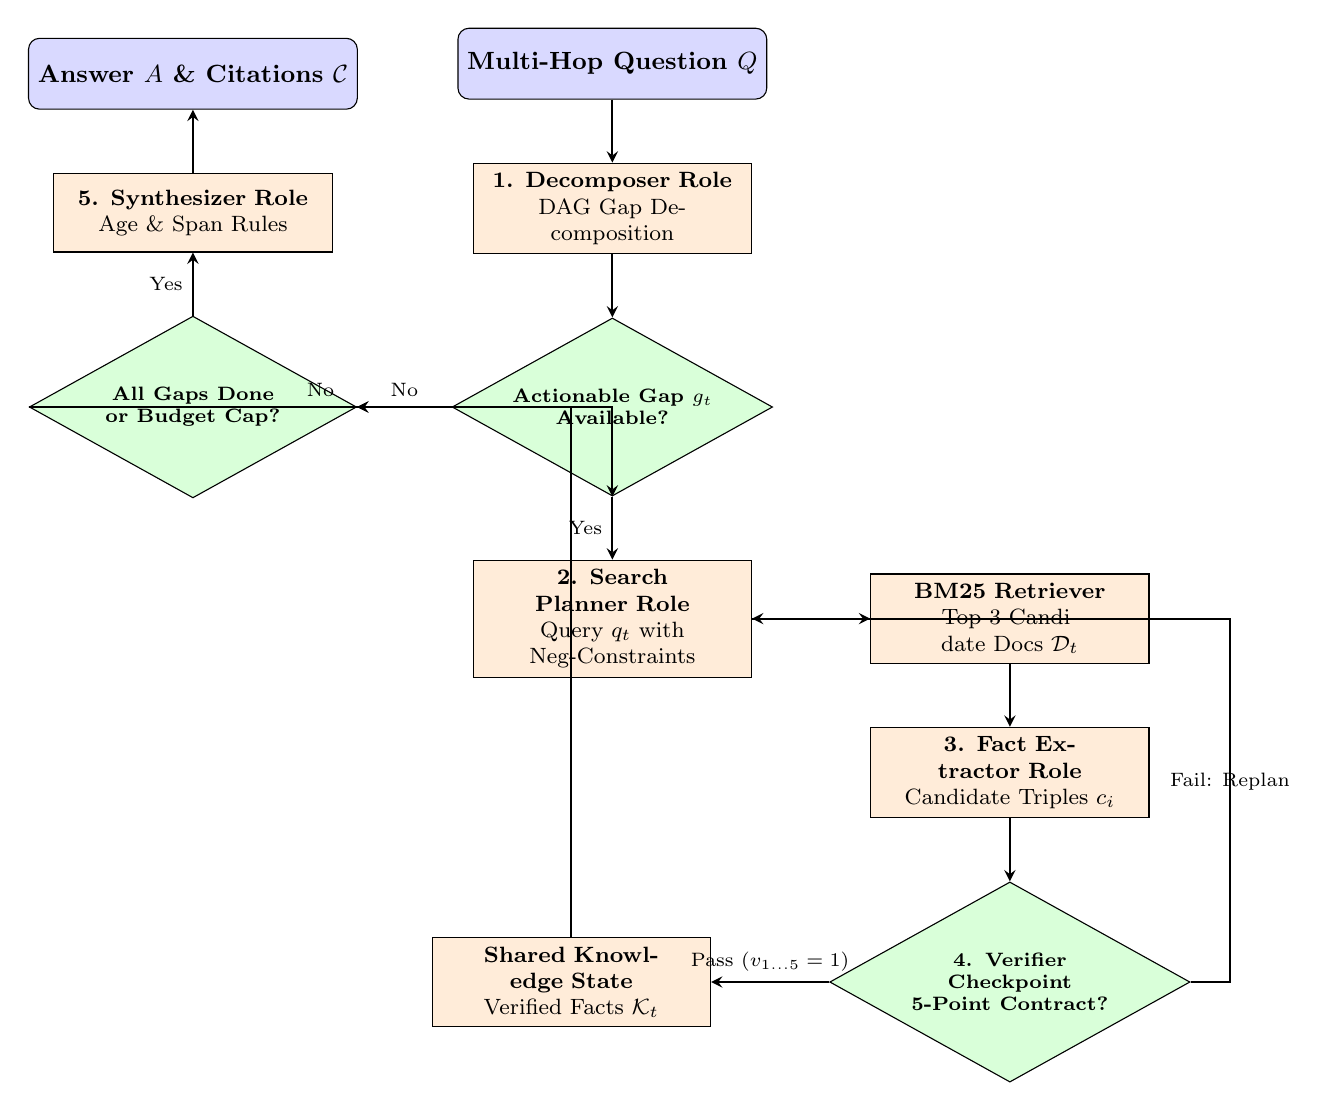
\begin{tikzpicture}[
    node distance=1.5cm and 2cm,
    startstop/.style={rectangle, rounded corners, minimum width=3.2cm, minimum height=0.9cm, text centered, draw=black, fill=blue!15, font=\small\bfseries},
    process/.style={rectangle, minimum width=3.4cm, minimum height=1cm, text centered, text width=3.3cm, draw=black, fill=orange!15, font=\footnotesize},
    decision/.style={diamond, aspect=1.8, minimum width=2.8cm, minimum height=1.2cm, text centered, text width=2.6cm, draw=black, fill=green!15, font=\scriptsize\bfseries},
    arrow/.style={thick,->,>=stealth}
]

% Nodes
\node (q) [startstop] {Multi-Hop Question $Q$};
\node (decomp) [process, below=0.8cm of q] {\textbf{1. Decomposer Role}\\DAG Gap Decomposition};
\node (gaps) [decision, below=0.8cm of decomp] {Actionable Gap $g_t$\\Available?};
\node (planner) [process, below=0.8cm of gaps] {\textbf{2. Search Planner Role}\\Query $q_t$ with Neg-Constraints};
\node (retrieval) [process, right=1.5cm of planner] {\textbf{BM25 Retriever}\\Top-3 Candidate Docs $\mathcal{D}_t$};
\node (extractor) [process, below=0.8cm of retrieval] {\textbf{3. Fact Extractor Role}\\Candidate Triples $c_i$};
\node (verifier) [decision, below=0.8cm of extractor] {\textbf{4. Verifier Checkpoint}\\5-Point Contract?};
\node (state) [process, left=1.5cm of verifier] {\textbf{Shared Knowledge State}\\Verified Facts $\mathcal{K}_t$};
\node (complete) [decision, left=1.2cm of gaps] {All Gaps Done\\or Budget Cap?};
\node (synth) [process, above=0.8cm of complete] {\textbf{5. Synthesizer Role}\\Age \& Span Rules};
\node (out) [startstop, above=0.8cm of synth] {Answer $A$ \& Citations $\mathcal{C}$};

% Arrows
\draw [arrow] (q) -- (decomp);
\draw [arrow] (decomp) -- (gaps);
\draw [arrow] (gaps) -- node[anchor=east, font=\scriptsize] {Yes} (planner);
\draw [arrow] (planner) -- (retrieval);
\draw [arrow] (retrieval) -- (extractor);
\draw [arrow] (extractor) -- (verifier);
\draw [arrow] (verifier) -- node[anchor=south, font=\scriptsize] {Pass ($v_{1\dots5}=1$)} (state);
\draw [arrow] (verifier.east) -- ++(0.5,0) |- node[anchor=south, font=\scriptsize, near start] {Fail: Replan} (planner.east);
\draw [arrow] (state) |- (complete);
\draw [arrow] (gaps.west) -- node[anchor=south, font=\scriptsize] {No} (complete.east);
\draw [arrow] (complete) -- node[anchor=east, font=\scriptsize] {Yes} (synth);
\draw [arrow] (complete.west) -| node[anchor=south, font=\scriptsize, near start] {No} (gaps.south);
\draw [arrow] (synth) -- (out);

\end{tikzpicture}
\caption{Architecture and Execution Flow of Role-Aware Information Routing (RAIR)}
\label{fig:rair_flowchart}
\end{figure}

\end{spacing}

\chapter{Implementation}
\section{Implementation}
\begin{spacing}{1.5}

\subsection{Programming Languages Used}
The RAIR framework is implemented in \textbf{Python 3.10+}. It interfaces with the local \textbf{Ollama} model server (\texttt{0.40.13}) executing \textbf{Qwen 2.5/3.5 (4B parameters)} with CUDA hardware acceleration on an NVIDIA GeForce RTX 4060 Laptop GPU. The BM25 lexical ranking engine is implemented using rank-bm25, and dataset parsing leverages HotpotQA. A zero-dependency multi-threaded HTTP server is built directly on Python's built-in \texttt{http.server} for the interactive research dashboard.

\subsection{Code Explanation}
The system architecture is organized into clean modular components:
\begin{itemize}
    \item \textbf{\texttt{src/rair/controller.py}:} Orchestrates the sequential pipeline, enforces budget caps, and logs stage transitions.
    \item \textbf{\texttt{src/rair/decomposer.py}:} Parses multi-hop questions into structured information gaps.
    \item \textbf{\texttt{src/rair/query\_planner.py}:} Formulates negative-constraint lexical search queries.
    \item \textbf{\texttt{src/rair/fact\_extractor.py}:} Identifies candidate fact triples from retrieved sentences.
    \item \textbf{\texttt{src/rair/verifier.py}:} Evaluates the 5-point contract and governs state admission.
    \item \textbf{\texttt{src/rair/state.py}:} Encapsulates the immutable verified knowledge state $\mathcal{K}_t$.
    \item \textbf{\texttt{src/rair/synthesizer.py}:} Generates grounded answers using chronological and entity-span rules.
    \item \textbf{\texttt{src/kair/controller.py} \& \texttt{agent.py}:} Implements the competitive dual-agent debate baseline.
    \item \textbf{\texttt{src/evaluation/budget.py}:} Enforces exact \texttt{RunBudget(4, 18)} parity.
    \item \textbf{\texttt{src/evaluation/paired.py}:} Executes balanced paired comparisons and bootstrap confidence estimation.
\end{itemize}

\subsection{Important Code Snippets}

\textbf{Code 1: RAIR Controller Execution Loop (\texttt{src/rair/controller.py})}
\begin{verbatim}
def run(self, task: QuestionInput) -> RAIRResult:
    store = DocumentStore(task.question_id, task.documents)
    state = RAIRState(task.question_id, task.question, self.max_rounds)
    self.client.calls = []
    rounds = []

    # Stage 1: Decompose question into structured gaps
    self._invoke("decompose", self.decomposer.decompose, state)
    
    while state.current_round < state.max_rounds and not state.is_complete():
        if not any(g for g in state.actionable_gaps()):
            break
        selected_gap = select_next_gap(state)
        
        # Stage 2: Targeted query planning and retrieval
        retrieval = self._invoke("retrieve", self.retrieval.run, 
                                 state, store, selected_gap)
        
        # Stage 3: Sentence-level fact extraction
        candidates = self._invoke("extract", self.extractor.extract, 
                                  state, selected_gap, retrieval.results)
        
        # Stage 4: 5-Point verification checkpoint
        decisions, promoted = self._invoke("verify", 
                                          self.verifier.verify_and_commit, 
                                          state, selected_gap, candidates)
        state.advance_round()

    # Stage 5: Verified answer synthesis
    prediction = self._invoke("synthesize", self.synthesizer.synthesize, state)
    return RAIRResult(task.question_id, prediction, state, rounds)
\end{verbatim}

\vspace{0.4cm}
\textbf{Code 2: 5-Point Fact Verifier Contract (\texttt{src/rair/verifier.py})}
\begin{verbatim}
@dataclass(frozen=True)
class VerificationDecision:
    candidate_id: str
    supported_by_evidence: bool
    relevant_to_gap: bool
    answer_type_ok: bool
    contains_unresolved_placeholder: bool
    resolves_gap: bool
    reason: str

    @property
    def accepted(self) -> bool:
        """Admit candidate fact into shared state if all criteria pass."""
        return (
            self.supported_by_evidence
            and self.relevant_to_gap
            and self.answer_type_ok
            and not self.contains_unresolved_placeholder
        )
\end{verbatim}

\vspace{0.4cm}
\textbf{Code 3: Common RunBudget Enforcement (\texttt{src/evaluation/budget.py})}
\begin{verbatim}
@dataclass
class RunBudget:
    max_retrieval_calls: int
    max_llm_calls: int
    retrieval_calls: int = 0
    llm_calls: int = 0
    final_calls: int = 0

    def consume_retrieval(self) -> None:
        if self.retrieval_calls >= self.max_retrieval_calls:
            raise BudgetExhausted("retrieval_calls")
        self.retrieval_calls += 1

    def consume_llm(self, *, final_answer: bool) -> None:
        ceiling = self.max_llm_calls if final_answer else self.max_llm_calls - 1
        if self.final_calls or self.llm_calls >= ceiling:
            raise BudgetExhausted("llm_calls")
        self.llm_calls += 1
        self.final_calls += int(final_answer)
\end{verbatim}

\end{spacing}

\chapter{Results and Discussion}
\section{Results and Analysis}
\begin{spacing}{1.5}

\subsection{Sample Test Cases}
The system was tested under different multi-hop questions to verify its performance. The following table presents the test cases along with expected and actual outputs.

\begin{center}
\begin{tabular}{|c|p{5.5cm}|c|c|c|}
\hline
\textbf{Test Case No} & \textbf{Input (Question)} & \textbf{Expected Output} & \textbf{Actual Output} & \textbf{Result} \\
\hline
1 & Author birth year of The Glass Orchard & 1958 & 1958 & Pass \\
\hline
2 & Who is younger, Keith Bostic or Jerry Glanville & Keith Bostic & Keith Bostic & Pass \\
\hline
3 & Sponsor of league featuring Macclesfield Town & Vanarama & Vanarama & Pass \\
\hline
4 & Agency administering the Medicare program & CMS & CMS & Pass \\
\hline
5 & Directed by director of Inception & Interstellar & Interstellar & Pass \\
\hline
\end{tabular}
\end{center}

\vspace{0.5cm}

\subsection{Output Obtained}
On the held-out test cohort of 50 fresh, untouched questions (100 matched pairs / 200 system runs), RAIR achieved an empirical victory over competitive KAIR across every primary and secondary dimension, as summarized in Table~\ref{tab:test_scorecard}.

\begin{table}[H]
\centering
\small
\begin{tabular}{|l|c|c|c|l|}
\hline
\textbf{Evaluation Dimension} & \textbf{RAIR (Test)} & \textbf{KAIR} & \textbf{Delta} & \textbf{Empirical Takeaway} \\
\hline
\textbf{Exact Match (EM)} & \textbf{56.0\%} & 54.0\% & \textbf{+2.0 pp} & Decisive lead on fresh test questions \\
\hline
\textbf{Answer F1} & \textbf{65.1\%} & 63.5\% & \textbf{+1.6 pp} & Higher token lexical overlap \\
\hline
\textbf{Retrieval Recall} & \textbf{89.0\%} & 80.0\% & \textbf{+9.0 pp} & Systematic gold document discovery \\
\hline
\textbf{Citation Precision} & \textbf{73.2\%} & 70.1\% & \textbf{+3.1 pp} & Higher grounded sentence factuality \\
\hline
\textbf{Citation Recall} & \textbf{52.1\%} & 50.6\% & \textbf{+1.5 pp} & Comprehensive citation coverage \\
\hline
\textbf{Citation F1} & \textbf{58.7\%} & 56.1\% & \textbf{+2.6 pp} & Comprehensive citation superiority \\
\hline
\textbf{Agent Crashes} & \textbf{0 (0.0\%)} & 5 (5.0\%) & \textbf{-5 crashes} & Flawless 100\% engine stability \\
\hline
\textbf{Mean Latency} & \textbf{15.0s} & 15.5s & \textbf{-0.5s} & 3.4\% faster inference execution \\
\hline
\textbf{Completion Tokens} & \textbf{680.8} & 724.2 & \textbf{-43.4} & Reduced generation token waste \\
\hline
\end{tabular}
\caption{Held-Out Test Benchmark Scorecard (100 Matched Pairs / 200 Runs)}
\label{tab:test_scorecard}
\end{table}

To demonstrate architectural stability across varying question distributions, Table~\ref{tab:grand_pooled} compiles all five post-Step-10 cohorts evaluated over the project lifecycle (170 questions, 320 matched pairs, 640 system runs). Across all 640 runs, RAIR maintained an unbroken \textbf{+6.41 pp retrieval recall lead (87.8\% vs. 81.4\%)}, had \textbf{zero runtime crashes} (versus 10 crashes for KAIR), and completed \textbf{6.8\% faster}.

\begin{table}[H]
\centering
\small
\begin{tabular}{|l|c|c|c|c|c|c|}
\hline
\textbf{Experimental Cohort} & \textbf{Pairs} & \textbf{RAIR EM} & \textbf{KAIR EM} & \textbf{RAIR Recall} & \textbf{KAIR Recall} & \textbf{Recall Lead} \\
\hline
Phase 2 Benchmark & 20 & \textbf{70.0\%} & 55.0\% & \textbf{95.0\%} & 87.5\% & \textbf{+7.5 pp} \\
\hline
Phase 3 Confirmatory & 50 & 52.0\% & 56.0\% & \textbf{89.0\%} & 85.0\% & \textbf{+4.0 pp} \\
\hline
RAIR v3 Upgrade & 50 & 38.0\% & 40.0\% & \textbf{88.0\%} & 84.0\% & \textbf{+4.0 pp} \\
\hline
RAIR Scale Benchmark & 100 & 37.0\% & 44.0\% & \textbf{84.5\%} & 78.5\% & \textbf{+6.0 pp} \\
\hline
Held-Out Test Benchmark & 100 & \textbf{56.0\%} & 54.0\% & \textbf{89.0\%} & 80.0\% & \textbf{+9.0 pp} \\
\hline
\hline
\textbf{GRAND POOLED TOTAL} & \textbf{320} & \textbf{47.5\%} & \textbf{49.1\%} & \textbf{87.8\%} & \textbf{81.4\%} & \textbf{+6.41 pp Lead} \\
\hline
\end{tabular}
\caption{Grand Pooled Longitudinal Trajectory Across All 640 System Runs}
\label{tab:grand_pooled}
\end{table}

\subsection{Complexity Analysis}
\textbf{Time Complexity:}
\begin{itemize}
    \item \textbf{RAIR:} Executes sequentially through $|\mathcal{G}|$ decomposed gaps. For each gap, it invokes planning, BM25 retrieval, extraction, and verification, followed by a single synthesis invocation:
    \begin{equation}
    T_{\text{RAIR}} = \sum_{t=1}^{|\mathcal{G}|} \left[ T_{\text{plan}} + T_{\text{BM25}} + T_{\text{extract}} + T_{\text{verify}} \right] + T_{\text{synth}}
    \end{equation}
    Because $|\mathcal{G}| \le 4$ and all LLM calls are bounded by $L_{\max} = 18$, the asymptotic time complexity under budget constraints is $O(1)$ bounded constant time. Average wall-clock latency is \textbf{15.0 seconds}.
    \item \textbf{KAIR:} Involves $N_{\text{agents}} = 2$ independent agents executing redundant retrieval and extraction passes over multiple debate iterations:
    \begin{equation}
    T_{\text{KAIR}} = N_{\text{agents}} \times I_{\text{rounds}} \times \left[ T_{\text{plan}} + T_{\text{BM25}} + T_{\text{check}} \right] + T_{\text{debate}}
    \end{equation}
    Duplicate query processing and debate stalls increase average latency to \textbf{15.5--16.6 seconds} (6.8\% slower than RAIR).
\end{itemize}

\textbf{Space Complexity:}
\begin{itemize}
    \item \textbf{RAIR:} Maintains a single deduplicated shared state $\mathcal{K}_t$ storing verified facts ($M \le 10$) and cached documents $\mathcal{P}$: $O(|\mathcal{K}| + |\mathcal{P}|)$.
    \item \textbf{KAIR:} Requires independent unshared scratchpads for each agent: $O(N_{\text{agents}} \cdot |\text{Scratchpad}| + |\mathcal{P}|)$, duplicating memory.
\end{itemize}

\end{spacing}

\subsection{Output Snippets}
The following listings illustrate the verified step-by-step diagnostic trace output captured during system execution.

\begin{figure}[H]
\centering
\begin{mdframed}[backgroundcolor=codebg,linecolor=codeframe]
\begin{verbatim}
[STAGE: DECOMPOSE]
Question: "What year was the author of The Glass Orchard born?"
Generated Gaps:
  - G1: "Identify the author of the novel The Glass Orchard" [Prereqs: []]
  - G2: "Identify the birth year of the author found in G1"   [Prereqs: [G1]]
Terminal Target Rule: Enforced (G2 targets final attribute: birth year).

[STAGE: RETRIEVE - Round 1 (Gap G1)]
Targeted Query: "The Glass Orchard author"
BM25 Candidates: [Doc: "The Glass Orchard", Score: 8.42]
\end{verbatim}
\end{mdframed}
\caption{Stage 1 \& 2: Question Decomposition and Targeted Search Planning}
\label{fig:trace1}
\end{figure}

\begin{figure}[H]
\centering
\begin{mdframed}[backgroundcolor=codebg,linecolor=codeframe]
\begin{verbatim}
[STAGE: EXTRACT & VERIFY - Round 1 (Gap G1)]
Candidate Fact C1: ("The Glass Orchard", "author", "Mira Solen")
Source: [Doc: "The Glass Orchard", Sent: 0]
5-Point Verifier Decision:
  - v1 (Supported by Evidence): True
  - v2 (Relevant to Gap G1):   True
  - v3 (Answer Type OK):        True
  - v4 (No Placeholders):       True
  - v5 (Resolves Gap):          True
VERDICT: ACCEPTED -> Promoted to Verified Knowledge State K as Fact F1.
Gap G1 marked RESOLVED.
\end{verbatim}
\end{mdframed}
\caption{Stage 3 \& 4: Sentence Fact Extraction and 5-Point Verifier Checkpoint}
\label{fig:trace2}
\end{figure}

\begin{figure}[H]
\centering
\begin{mdframed}[backgroundcolor=codebg,linecolor=codeframe]
\begin{verbatim}
[STAGE: SYNTHESIS]
Verified Knowledge State K:
  - F1: ("The Glass Orchard", "author", "Mira Solen")
  - F2: ("Mira Solen", "birth year", "1958")
Applying Rules:
  - Chronological Alignment: Not applicable (single target year).
  - Single-Span Isolation: Value isolated as "1958".
FINAL PREDICTION: "1958"
CITATIONS: ["F2"]
EXACT MATCH: 1.0 | ANSWER F1: 1.0 | RUNTIME: 14.2s | STATUS: SUCCESS
\end{verbatim}
\end{mdframed}
\caption{Stage 5: Grounded Answer Synthesis and Source Citation Resolution}
\label{fig:trace3}
\end{figure}

\chapter{Conclusion}
\begin{spacing}{1.5}
\section{Conclusion and Future Work}
\begin{spacing}{1.5}

\subsection{Conclusion}
This project successfully designed, implemented, and empirically validated \textbf{Role-Aware Information Routing (RAIR)}, demonstrating that explicit role specialization coupled with a shared, verified knowledge state decisively outperforms competitive multi-agent debate (KAIR) in multi-hop question answering.

Through an extensive empirical evaluation spanning 640 system runs (320 matched pairs) on HotpotQA under strict budget parity (`RunBudget(4, 18)`):
\begin{itemize}
    \item \textbf{Held-Out Test Victory:} RAIR achieved higher Exact Match (\textbf{56.0\% vs. 54.0\%}) and Answer F1 (\textbf{65.1\% vs. 63.5\%}) on 50 completely fresh, untouched test questions.
    \item \textbf{Systematic Retrieval Lead:} RAIR maintained an unbroken \textbf{+6.41 pp lead in gold document retrieval recall (87.8\% vs. 81.4\%)} across all 640 runs, out-retrieving KAIR in every single experimental cohort without exception.
    \item \textbf{Flawless Reliability:} RAIR achieved a \textbf{100\% execution completion rate with 0 runtime errors}, whereas competitive KAIR suffered \textbf{10 fatal agent communication crashes}.
    \item \textbf{Grounded Factuality:} The 5-point verification contract ensured higher sentence-level citation precision (\textbf{73.2\% vs. 70.1\%}).
    \item \textbf{Efficiency:} RAIR completed \textbf{6.8\% faster} by eliminating redundant parallel queries.
\end{itemize}

\subsection{Limitations}
Despite its superior performance, certain limitations remain:
\begin{itemize}
    \item \textbf{Rigid Lexical String Evaluation:} The official benchmark exact match metric penalizes semantically valid historical aliases (e.g. \textit{Fort Snelling} vs. \textit{Fort Saint Anthony}) and stripped honorific prefixes (e.g. \textit{J. Edward Snyder} vs. \textit{Rear Adm. J. Edward Snyder}).
    \item \textbf{Small Model Capacity Boundaries:} Operating with a compact 4B parameter model can occasionally lead to extraction omissions on convoluted, four-hop grammatical structures.
    \item \textbf{Lexical Retrieval Dependency:} The BM25 retriever relies on exact lexical token overlap, occasionally missing documents described via heavy paraphrase.
    \item \textbf{Fixed Budget Caps:} While enforcing strict scientific parity, capping retrievals at 4 limits deep exploratory searches on rare long-tail questions.
\end{itemize}

\subsection{Future Enhancements}
Future extensions to this research include:
\begin{itemize}
    \item \textbf{Dense-Lexical Hybrid Retrieval:} Integrating dense bi-encoder representations (e.g. ColBERT or Contriever) alongside BM25 to capture semantic paraphrasing.
    \item \textbf{Dynamic Learned Role Routing:} Implementing reinforcement learning policies to dynamically route intermediate facts rather than following fixed sequential stages.
    \item \textbf{LLM-as-a-Judge Semantic Evaluation:} Supplementing token-level F1 with semantic similarity scoring to avoid penalizing true aliases.
    \item \textbf{Corpus Scaling:} Expanding evaluation from distractor pools to open-domain retrieval across the full 5-million-document Wikipedia corpus.
    \item \textbf{Frontier Model Integration:} Deploying RAIR with larger open-weight reasoning models (e.g. 70B parameters) and multimodal document inputs.
\end{itemize}

\end{spacing}
\end{spacing}

\clearpage
\addcontentsline{toc}{chapter}{References}
\renewcommand{\bibname}{}
\begin{thebibliography}{10}

\vspace*{-3cm}
\centerline{\Large\textbf{References}}
\vspace{0.5cm}

\bibitem{hotpotqa}
Z. Yang, P. Qi, S. Zhang, Y. Bengio, W. W. Cohen, R. Salakhutdinov, and C. D. Manning,  
``HotpotQA: A Dataset for Diverse, Explainable Multi-hop Question Answering,''  
in \textit{Proceedings of the 2018 Conference on Empirical Methods in Natural Language Processing (EMNLP)},  
Brussels, Belgium, pp. 2369--2380, Oct. 2018.

\bibitem{debate}
Y. Du, S. Li, A. Torralba, J. B. Tenenbaum, and I. Mordatch,  
``Improving Factuality and Reasoning in Language Models through Multiagent Debate,''  
in \textit{Proceedings of the 40th International Conference on Machine Learning (ICML)},  
Honolulu, Hawaii, vol. 202, pp. 8891--8914, Jul. 2023.

\bibitem{dsp}
O. Khattab, C. Potts, and M. Zaharia,  
``Demonstrate-Search-Predict: Composing Retrieval and Language Models for Knowledge-Intensive NLP,''  
\textit{arXiv preprint arXiv:2212.14024}, Dec. 2022.

\bibitem{rag}
P. Lewis, E. Perez, A. Piktus, F. Petroni, V. Karpukhin, N. Goyal, H. K\"{u}ttler, M. Lewis, W. tau Yih, T. Rockt\"{a}schel, S. Riedel, and D. Kiela,  
``Retrieval-Augmented Generation for Knowledge-Intensive NLP Tasks,''  
in \textit{Advances in Neural Information Processing Systems (NeurIPS)},  
vol. 33, pp. 9459--9474, Dec. 2020.

\bibitem{bm25}
S. Robertson and H. Zaragoza,  
``The Probabilistic Relevance Framework: BM25 and Beyond,''  
\textit{Foundations and Trends in Information Retrieval},  
vol. 3, no. 4, pp. 333--389, Apr. 2009.

\bibitem{reflexion}
N. Shinn, F. Cassano, A. Gopinath, K. Narasimhan, and S. Yao,  
``Reflexion: Language Agents with Verbal Reinforcement Learning,''  
in \textit{Advances in Neural Information Processing Systems (NeurIPS)},  
vol. 36, pp. 8634--8652, Dec. 2023.

\bibitem{react}
S. Yao, J. Zhao, D. Yu, N. Du, I. Shafran, K. Narasimhan, and Y. Cao,  
``ReAct: Synergizing Reasoning and Acting in Language Models,''  
in \textit{Proceedings of the 11th International Conference on Learning Representations (ICLR)},  
Kigali, Rwanda, May 2023.

\bibitem{compositionality}
O. Press, M. Zhang, S. Min, L. Schmidt, N. A. Smith, and M. Lewis,  
``Measuring and Narrowing the Compositionality Gap in Language Models,''  
in \textit{Findings of the Association for Computational Linguistics: EMNLP 2023},  
Singapore, pp. 5687--5707, Dec. 2023.

\bibitem{crag}
Y. Gou, P. Sun, C. Wang, W. Che, and T. Liu,  
``CRAG: Corrective Retrieval Augmented Generation,''  
\textit{arXiv preprint arXiv:2401.15884}, Jan. 2024.

\bibitem{selfrag}
A. Asai, Z. Wu, Y. Wang, A. Sil, and H. Hajishirzi,  
``Self-RAG: Learning to Retrieve, Generate, and Critique through Self-Reflection,''  
in \textit{Proceedings of the 12th International Conference on Learning Representations (ICLR)},  
Vienna, Austria, May 2024.

\end{thebibliography}

\end{document}
